\documentclass{article}
\usepackage{amsmath}
\usepackage{listings}
\usepackage{amssymb}
\usepackage{color}
\usepackage{graphicx}
\graphicspath{ {images/} }
\usepackage[margin=1.15in]{geometry}

\lstset{frame=tb,
  basicstyle=\footnotesize,
  language=C,
  aboveskip=2mm,
  belowskip=2mm,
  frame=none,
  keepspaces=true,
  showstringspaces=false,
  columns=flexible,
  basicstyle={\small\ttfamily},
  breaklines=false,
  breakatwhitespace=false,
  tabsize=2
}

\lstset{language=C}

\title{DTOADQ}

\begin{document}
  \maketitle
  \section{Introduction}

  \section{Signed Distance Fields}
  Signed Distance Fields (SDFs) are a mathematical tool to represent a 3D primitive by describing its surface via a distance field. Given an arbitrary point in space, the SDF of a primitive is the distance to its nearest point/surface. For example, the SDF of a sphere is $\Vert\:O\:\Vert - R$. With SDFs, it's possible to march a ray along the scene until it hits the surface of an SDF within a given bound, using the returned SDF distance as the distance to march. Some example SDFs are shown below:    \begin{align*}
  S(P, R) &= \Vert\:P\:\Vert - R & \text{Sphere with Radius}\\
  S(P, N) &= P \cdot N  & \text{Plane with Normal}\\
  S(P, H, R) &= <\Vert\:P_{x, z}\:\Vert - R, \: P_{y}> - H & \text{Torus with Radius and Hole}\\
  \end{align*}
  
  The biggest issue with SDFs is Lipschitz continuity. The SDFs themselves have a distance gradient, that is, their bound. The bounds of a SDF is expected to be at most 1 in order to remain Lipschitz continuous, as otherwise the SDF will appear deformed as shown below.
  
  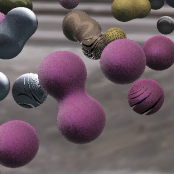
\includegraphics[]{lipschittzbound}
  
  This is a larger problem in Light Transport than it is in raytracing because small discontinuities can impact the lighting of an entire scene. And to add to that, most interesting operations (such as the meta balls shown in the image above) will violate Lipschitz. The easiest way to fix this is to multiply the distance field by a constant to stay below 1, but this is less of a fix and more of a hack.
  
  
  In order to compute a normal of an SDF, you must perform a gradient approximation: the central distance onf the SDF at
  P. For example, the difference quotient:
  \[\frac{(f(x+h) - f(x))}{h}\]

  \section{OpenCL}
	OpenCL, and GPU programming in general, is where I am least knowledgeable or interested. Well, OpenCL is easy to work with, and I wrote my own OpenCL module to handle OCL in a rather convenient method, for example, the DTOADQ kernel call looks as such:
	\begin{lstlisting}
	shared_info.image.Lock(); // Acquire OCL Mem from OGL image object
	ocl.Run(
	  ocl.CLStoreMem(shared_info.rw_image),
	  shared_info.image.RWrite(),
	  ocl.CLStoreMem(shared_info.image_metadata),
	  shared_info.camera,
	  shared_info.timer,
	  ocl.CLPredefinedMem(imgs),
	  ocl.CLStoreMem(shared_info.ocl_material),
	  debug_values,
	  ocl.CLStoreMem(shared_info.rng_states),
	  // kernel size
	  shared_info.image.x, shared_info.image.y
	);
	shared_info.image.Unlock();
	
	\end{lstlisting}
	
	however the problem comes with dealing with the intrinsics of GPU; optimizing code for the GPU and knowing how memory and threads/workers are handled.
  
  	One benefit of OpenCL is its ease to debug in comparison to OpenGL. One immediate benefit is printf, which surprisingly even works on the GPU. To make printf easily readable, I only use print on the center pixel of the image. Even so, due to the complexity of light transport, the vast majority of time spent on this project went directly towards debugging the DTOADQ kernel.
  	
  	OpenCL also makes it relatively easy to send and receive data between the host and GPU. In comparison to OpenGL, this is a big win, however, with OpenGL4.3's Shader Storage Buffer Object, this is now no longer a selling point.
  	
  	OpenCL also has huge drawbacks. The biggest problem is getting the results to be rendered in OpenGL. TODO. Also, there are minor annoyances, like the lack of a matrix data type, no function overloads, long compile times, or variadic functions. There are also annoyances with GPU programming in general. No dedicated random function. Though, possibly, long compile times is my fault for using a mega-kernel instead of splitting it into many small kernels.
  	
  	It seems that the GPU is not for me or DTOADQ and something I do not enjoy to use nor am good at. However, for this project, I had to deal with it. To overcome the lack of a random function, of which high quality uniform random generation is necessary for Monte Carlo simulations, I used the MWC64X algorithm. While there are better algorithms, they fail on branches which makes it useless for DTOADQ. It seemed to work well enough. The downside is that each worker/pixel needs its own random state, preserved across multiple kernel calls. There are indefinitely better solutions.
  \section{Light Transport Introduction}
  \section{Bidirectional Path Tracing}
    The main foundation of the mathematics and theory have come from many sources, from Veach's PhD thesis to PBR 3rd ed. and various open source path tracing kernels such as NanoRT, Embree, etc. However, the implementation differs from these in that the algorithm is optimized for the GPU. This section is about transforming the algorithms and mathematical models from Veach's thesis into something easily and efficiently implementable the GPU.

    Calculating probability distribution functions is a very vital component in
    Monte Carlo Sampling. The PDF states the probability of a random variable to
    take the form of a given input. Its usefulness comes when contributions from
    many Monte Carlo samples have a different weight. That is, one sample may
    have a higher probability distribution, and thus a higher contribution to
    the path. That's the strategy behind Monte Carlo;
    \begin{align}
      \int f(x) \approx \frac{1}{N}\Sigma_0^N\frac{f(x)}{p(x)}
    \end{align}
    The PDF applies to everything from path contributions, solid angles of a
    BRDF, uniformly sampling a sphere, etc. I had a difficult time understanding
    these, and more importantly, how to calculate them for a given formula. The
    biggest conceptual barrier is that, for example, given a solid angle in a
    hemisphere $\Omega$, the probability for a random uniform $X$ to equal
    $\omega$ is 0. That's not what the PDF calculates, instead, it's the
    probability that a random uniform $X$ could potentially equal $\omega$ when compared to other $\omega\:$s. In other words, it's about comparing the probability of $X$ to equal $\omega$ when compared to another theoretical z$\omega$.

    The good thing is that calculating these are relatively easy. There's a
    reliable three-step process. The first is to
    find the cumulative distribution function $CDF = Pr(X \leq x)$. Where $Pr$
    is the probability, $X$ is a uniformly random variable, and $x$ is a known
    constant. In other words, this gives the probability that, for a formula
    $P$, where $X \in \Omega$, and $\Omega$ is the set of all possible values
    for $CDF$,
    that $X \leq x$. The second step is to take the derivative of this, so for
    PDF $p$
    \begin{align}
      p(x) = \frac{dCDF(x)}{dx}
    \end{align}
    And the final step is to verify that the PDF is correct by integrating it
    over $\Omega$, this final value should equal 1. This makes sense intuitively
    -- it is a probability after all, so the sum of the probabilities of every
    possible input must be 1.
    For an example, how I calculated the PDF of an area light source
      $L^0_e(v) = L_o(P, \omega_o)$ 
    is quite simple. Firstly,the area light is defined as a sphere, and thus our
    set of all possible values is correlated to surface area:
    $\Omega = [0,\:2.0f*\tau*R^2]$. Thus,
    \begin{align}
      CDF(x) = Pr(X \leq x) = \frac{x}{2.0*\tau*R^2}\\
      p(x) = \frac{dCDF(x)}{dx} = \frac{1.0}{2.0*\tau*R^2}\\
      \int_0^{\Omega}p(x)dx = 1.0
    \end{align}
    In code
    \begin{lstlisting}
      float Light_PDF ( Emitter* m ) {
        return 1.0f/(2.0f*TAU*SQR(m->radius));
      }
    \end{lstlisting}
    The more interesting aspect, in this example, is actually generating the
    uniformly distributed samples of a sphere. The naive method gives incorrect
    distributions.TODO {page 774}
    
    The most obvious way to calculate this is the six-point gradient; where for
    each axis you compute $f(x+h) - f(x-h)$, and normalize the result. This
    returns a vector pointing in the direction where the map's SDF changes the
    most: the normal. A four point gradient is possible; as long as each each
    point of the gradient is multiplied by $\epsilon$ before normalizing. The
    speedup from six to four is worthwhile, as computing each gradient is
    expensive as it involves a sdf map call. There are more utilities with
    gradients not yet currently provided in DTOADQ but are worth mentioning, a
    few are: an additional normal call using an alternative (higher-quality) SDF
    map can be used to compute a 'normal' bumpmap, and analyzing the gradient by
    hand allows a cheap normal computation of primitives such as a spheres.
  
    Rendering equation with solid angle:
  \begin{align}
    L_o(P, \omega_o) = L_o(P, \omega_o) + \int_{\Omega}f_s(P, \omega_i,
    \omega_o) L_i(P, \omega_i) cos\Theta_i d\omega_i
  \end{align}
    To get from solid angle to path, consider:
  \begin{align}
    f_s(v \rightarrow \dot{v} \rightarrow \ddot{v}) &= f_s(P, \omega_i,
                                                      \omega_o)\\
    L_e(v \rightarrow \dot{v}) &= L_e(P, \omega_o)\\
    L_e(v \rightarrow \dot{v}) &= L_e^0(v) L_e^1(v \rightarrow \dot{v})
  \end{align}
    That is, instead of looking at a point $P$ with an incoming and outgoing
    angle $(\omega_i,\:\omega_o)$, look at the path from $P_{-1}$ ($v$) to
    $P_{+1}$ ($\ddot{v}$). More accurately, it's the transport between
    three different surfaces of the scene. In terms of SDFs, the surface
    is every point on an SDF map where $|map| \leq \epsilon$. There's no longer
    any integration over a hemisphere with solid angle $\omega_i$, it's now over
    every single surface in the scene. This will be explained in detail later.
\\
    In the case of $L_e$,
    DTOADQ [at least, for now], only has support for area-light. Thus consider:

  \begin{align}
    L_e(P, \omega_o) &\equiv L_e(P) &\text{[ for area lights ]}\\
    L_e(v \rightarrow \dot{v}) &= L_e^0(v)&
  \end{align}

    The cos term, used for the projected solid angle in irradiance, no longer
    applies when dealing with area. This and $d\omega_i$ now become a
    generalized geometry term, G, that converts a PDF with respect to solid area
    using Jacobian mapping, which involves the inverse squared distance, and the
    cosine angle between the geometric normals at $v$ and $\dot{v}$:

  \begin{align}
    cos\theta_n = v \cdot N(v) \\
    G(v \leftrightarrow \dot{v}) = V(v \rightarrow \dot{v})
        \frac{(cos\theta_n cos\dot{\theta_n})}{|| v - \dot{v}||^2}
  \end{align}

    Where $V$ is the visibility test. Thus the rendering equation with respects
    to area is:
  \begin{align}
    L(v \rightarrow \dot{v}) = L_e(v \rightarrow \dot{v}) \int_ML(v \rightarrow
    \dot{v}) G(v\leftrightarrow \dot{v}) f_s(v\rightarrow \dot{v} \rightarrow
    \ddot{v}) d_A
  \end{align}
    where $A$ is the area on $M$, and $M$ is the union of all scene surfaces.
    This is known as the three-point form or the light transport equation. By
    recursively expanding$^{[1]}$, so that the three point form is integrated
    over every possible set of possible paths, this can be rewritten as the more
    usable format:
  \begin{align} I_j = \int_\Omega f_j(\bar{v}) d\mu(\bar{v}) \end{align}
    Where $\bar{v}$ is a path $z_0\rightarrow z_s \rightarrow y_t \rightarrow
    y_0 (eye \rightarrow light)$, $\Omega$ is the combination of all possible
    paths of any length, and $\mu$ is the area-product measure [the product of
    all the expanded $d_A$]. Special care has to be taken with the definition of
    path itself, as in the source code, there never exists a path $\bar{v}$,
    only eye-path $\bar{z}$ and light-path . Right now, this is analytically
    unsolvable. To compute this, we need to apply monte carlo sampling and limit
    the maximum path length:
  \begin{align}
    I_j \approx \frac{1.0f}{N}\Sigma_0^NF\\
    F = \Sigma_s\Sigma_t\frac{f_j(\bar{v}_{s, t})}{p(\bar{v}_{s, t})}
  \end{align}

    where $s$ is the light-path length, and $t$ is the eye-path length. In
    DTOADQ, they are limited to $s+t \leq 8$[TODO]. Finally, to transform
    $\bar{v}$ into two seperate paths, $\frac{f_j(\bar{v}_{s,
        t})}{p(\bar{v}_{s, t})}$ is split into two with a connection edge $c$
  \begin{align}
    \frac{f_j(\bar{v}_{s, t})}{p(\bar{v}_{s, t})} \equiv
    \frac{f^L(\bar{y})}{p(\bar{y})} c(\bar{y}_s \leftrightarrow \bar{z}_t)
    \frac{f^E(\bar{z})}{p(\bar{z})}  
  \end{align}

    And now
  \begin{align}
    F = \Sigma_s\Sigma_t \alpha^L_s c_{s, t} \alpha^E_t
  \end{align}
  \begin{align}
    \alpha^{L|E}_i =
    \begin{cases}
      \frac{L_e^0(y_0 \rightarrow y_1)}{p_A(y_1)} | \frac{W^0_e(z_0)}{p_A(z_0)},
      &i = 1,\\
      (\frac{f_s(y_{i+1} \rightarrow y_i \rightarrow y_{i-1})}{p_{\sigma}(y_i
      \rightarrow y_{i-1})} | \frac{f_s(z_{i-1} \rightarrow z_{i-2} \rightarrow
      z_{i-3}}{p_\sigma(z_{i-2} \rightarrow z_{i-1})}) \alpha^{L|E}_{i-1},
      &i > 1
    \end{cases}
  \end{align}
    There is no case for $i = 0$ as either, the path doesn't exist, or if one
    does exist, $y_0$ and $z_0$ do not contribute to the image. Veach (and many other
    sources), leave this in, but it's unnecessarily confusing. A special case
    needs to be handled, unfortunately, for $\alpha^E_0$ as it is being
    generated on the fly while $\bar{z}$ is being constructed. The two options
    is to unroll the first iteration of the construction loop, or just allow the
    special case to exist. The latter is the better choice, as all kernels will
    enter and exit the special case at the same time, and the GPU might just
    unroll the loop anyways.
    There may be cases where $s = 0$ ($t = 0$ is not possible without a
    physical camera lens), which is equivalent to just forward path tracing.
    There is also to consider, what happens on $s = 1$ and $t = 1$, %TODO
    Well, in either case where both paths exist or only the camera path exists,
    the connection strategy below describes how to connect the edges of the two
    paths
  \begin{align}
    c_{s, t} =
    \begin{cases}
      L_e(z_{-2} \rightarrow z_{-1}), &s = 0, t > 1,\\
      f_s(y_{-2} \rightarrow y_{-1} \rightarrow z_{-1}) G(y_{-1} \leftrightarrow
      z_{-1}) f_s(y_{-1} \rightarrow z_{-1} \rightarrow z_{-2}), &s > 0, t > 1
    \end{cases}
  \end{align}
    Is the $s = 0, t > 1$
    strategy worthwhile to compute? Those familiar with next event
    estimation would know that there are situations in which this is beneficial.
    Take, for example, a glossy surface with a small solid angle subtending to
    the surface of a large light source. The $s=1$ sample strategy in this case
    would only contribute when the $L0$ vertex is within that solid angle.
    The effective strategy to sample in this case is $s = 0$.
    In code, $\alpha_i^E\:c_{s,t}\:\alpha_0^L$ looks like (MIS not shown):
    \begin{lstlisting}
     float3 wi = normalize(E1.origin - E0.origin),
            wo = normalize(L1.origin - E1.origin);
     float3 albedo = _BRDF_F(wi, E1.normal, wo, E1.material, E1.mat_col);
     albedo /= BSDF_PDF(wo, wi, &E1);
     Spectrum contribution = E1.radiance * albedo;
     contribution *= Geometric_Term(&E1, &L1, si, Tx);
     contribution *= tlight.emission/Light_PDF(&tlight);
    \end{lstlisting}
    
    Another question to consider is if the path should be able to reflect on the
    light source. While under real circumstances, this is allowed, the
    contribution is negligible and dismissed in DTOADQ. Also, there are no cases for $s = s, t = 0|1$ as
    the lens does not have a physical existence in the SDF map. The $t = 0$ case, where a photon from the light source hits the lens directly, is rather pointless anyways, as a path generated by light-tracing would have to be able to contribute to any pixel, which is not feasible on a GPU. The case of $t = 1$, where the light path is connected to a position on the lens, is important for effects such as depth of field and aperture. The only problem is due to time constraints, this has not been implemented yet.

    One immediately obvious optimization that could be made with this model is
    in regards to the visibility check in the geometric term, if you were to
    expand $I_j$, and take the V term from outside the G function
    [$G(v \rightarrow
    \dot{v}) V(v \rightarrow \dot{v})$],
    it would be made obvious that all the visibility checks can be
    cancelled out for the entire equation, except for the connection term $c$.
    This is intuitive as the paths
    $\bar{y}_{0} \ldots \bar{y}_s$ and $\bar{z}_0 \ldots \bar{z}_t$ had just been generated via raymarching.
    Specifically, the definition of $V$ is
  \begin{align}
    V(v \rightarrow \dot{v}) = ||v - \dot{v}|| \leq
    m(v,\:\overrightarrow{v\:\dot{v}})
  \end{align}
    where $m$ is a march through the SDF map. A visibility check is only
    necessary for the connection edge
    \begin{align*}
      ||v - \dot{v}|| = m(v, \overrightarrow{v, \dot{v}})\\
      \:\:\:\text{for all paths but } y_{-1} \rightarrow z_{-1} 
    \end{align*}
\\
    Moving on, for $\alpha^{L|E}_i$, these are equivalent for both $L$ and $E$,
    the problem is that the $\bar{y}$ path is generated in perspective of the
    light source, so there has to be a bit of caution in terms of perspective in when generating the PDFs.
    
     $p_A$ is
    the PDF w.r.t. area, for the light path; we only need to take the PDF of the
    solid angle of a sphere
  \begin{align}
    p_A^L(y_0 \rightarrow y_1) = p_{\sigma}^L(y_0 \rightarrow y_1) G(v
    \leftrightarrow \dot{v})\\
    p_{\sigma}^L(y_0 \rightarrow y_1) = \frac{1.0f}{\tau * (1.0f -
    \sqrt{\frac{R^2}{|y_0 - y_1|^2}})}
  \end{align}
    where $R$ is the radius of the sphere, note $y_0$ is a point on the surface
    of the sphere, and not its origin.
    \\$p_A^E(x_0 \rightarrow x_1)$ doesn't exist, as there is no physical lens
    on the scene. [TODO - this might cahnge later]. One of the benefits of this,
    is that there are no special cases for pathes where $t = 0$, which is
    impossible to handle on the GPU as the path could contribute to any
    arbitrary pixel [directly hitting the lens].
  \begin{align}
    P_A^E = 1.0f
  \end{align}
    The $L^0_e$ is contribution from the light source. As of right now, DTOADQ
    only supports area lights, so $L^0_e$ is set a constant for the emitter's
    spectrum value.
    The $W_e^0$ is contribution from the eye source, that is, the lens. Since
    the lens does not exist in the scene, as of now [TODO - this might change
    later], there is no $W_e^0$. While this should be implemented in the future,
    a hidden benefit of the current model is that there are no special cases for
    paths where $t = 0$, which is impossible to handle on the GPU as any such
    path could contribute to any arbitrary pixel [the light path is, after all,
    directly hitting the lens]. So this has now become:
  \begin{align}
    \alpha_i^E = \Sigma_{i\leq 0} 
  \end{align}
  The amount that each path contributes to F differ greatly, so naively
  weighing each contribution uniformly by something like 1.0f, or even, by
  inverse path length, will producy very noisy images, and would not be
  worth the additional computation time that BDPT requires, as shown below.
  	 To calculate the PDF of 
  In order to get good
  samples from the contributions, they must be combined in an optimal manner
  using Multiple Importance Sampling: each contribution is weighted by the PDF
  of the entire path itself:
  \begin{align*}
    F &\equiv \Sigma_s\Sigma_tW_{s, t}C_{s, t}\\
    C_{s, t} &= \alpha^L_s c_{s, t} \alpha^E_t
  \end{align*}
    where $W_{s, t}$ is the MIS weight of path $\bar{y} \leftarrow \bar{z}$, and
    $C_{s, t}$ is the unweighted contribution of the same path. For clarity,
    $C^U_{s, t}$ as described below is the unweighted contribution of the
    algorithm:
  \begin{align}
    C^u_{s, t} = (\alpha^L_s c_{s, t} \alpha^E_t) \equiv
    \frac{f_j(\bar{v})}{p(\bar{v})}
  \end{align}
  thus
  \begin{align}
    F = \Sigma_s\Sigma_tW_{s, t}C^u_{s, t}
  \end{align}
    The formula for Multiple Importance Sampling on BDPT is as so:
  \begin{align}
    MIS_{st}(\bar{x}) = \frac{P_s(\bar{x})}{\Sigma_i{P_i(\bar{x})}} 
  \end{align}
    Conceptually, the numerator $P_s(\bar{x})$ is the path density that was
    generated, while the denominator is the path density of other connection
    strategies that could could have, in theory,$^{[1]}$ created the path. The
    straight forward implementation of this has a lot of problems gone
    unresolved in Veach's thesis; PBR 3rd Ed, chapter 16 pg 1014-1016 addresses
    and describe these problems. Primarily, $P_i(\bar{x})$ will overflow
    CLFloat (due to the distance in the Geometric term), and the straight
    forward implementation is very long, hard to debug, and has a poor time
    complexity. But the important part is the end result of their solution:

  \begin{align}
    r_i (\bar{x}) = 
    \begin{cases}
      1.0f, & i = s,\\
      \frac{\overleftarrow{P}(\bar{x_i})}{\overrightarrow{P}(\bar{x_i})} *
      r_{i+1}(\bar{x}), & i < s,\\
      \frac{\overrightarrow{P}(\bar{x_{i-1}})}{\overleftarrow{P}(\bar{x_{i-1}})}
      * r_{i-1}(\bar{x}), & i > s
    \end{cases}
  \end{align}

    However, DTOADQ can simplify a bit further; unlike above, there are two
    paths for which to evaluate. Specifically, in the above term, for where
    $i < s$, we have
    $\frac{\overleftarrow{p}(\bar{x}_i)}{\overrightarrow{p}(\bar{x}_i)}$, 
    which is the light path (i is iterating towards light-length s). The eye
    contribution is inversed from this, (also iterating towards s, hence why
    $\bar{x}_{i-1}$ is used). Another way of saying it, is $\bar{x} = \bar{y} ||
    \bar{z}_{rev}$.
    In DTOADQ's case, the weights are calculated in
    the same direction relative to its originator; in this case the perspective
    of the eye path.
  \begin{align}
    \mathcal{W}_i(\bar{x}) \equiv r_i(\bar{x})\\
    \mathcal{W}_i (\bar{x}) = 
    \begin{cases}
      1.0f, & i = 0,\\
      \frac{\overleftarrow{p_i}(\bar{x_i})}{\overrightarrow{p_i}(\bar{x_i})} *
      \mathcal{W}_{i-1}(\bar{x}), & i > 0
    \end{cases}
  \end{align}
    And then the expanded form of $\mathcal{W}_i(\bar{x})$ looks like

  \begin{align}
    \mathcal{W}_i(\bar{x}) = \Pi_{n=2}^i(\frac{\overleftarrow
    {p_{\sigma}}(x_n)\overleftarrow {G}(x_n)}
    {\overrightarrow{p_{\sigma}}(x_n)\overrightarrow{G}(x_n)})
    * \frac{\overleftarrow{p_A}(x_1)}{\overrightarrow{p_A}(x_1)}
  \end{align}
 
    And now the MIS looks like:
  \begin{align}
    MIS_{s, t}(\bar{y}, \bar{z}) =
    \frac{1.0f}{\mathcal{W}_s(\bar{y}) + \mathcal{W}_t(\bar{z}) + 1.0f}
  \end{align}
    Thus, the final rendering equation for DTOADQ looks like such:

  \begin{align}
    P = \frac{1.0f}{N} \Sigma_{0}^{N} \Sigma_{s \le 0} \Sigma_{t \le 0}
    \alpha^L_s c_{s,t} \alpha^E_t MIS_{s, t}(\bar{y}, \bar{z})
  \end{align}


  \begin{align}
    P_i(\bar{x}_{s, t}) = P^L_s p^E_t
  \end{align}

  \begin{align}
    p^{L|E}_i(\bar{x}) =
    \begin{cases}
      1.0f, & i = 0,\\
      P_A(x_i), & i = 1,\\
      P_{\sigma}(x_{i-1} \rightarrow x_i) G(x_{i-1} \leftrightarrow x_i)
      P^{L|E}_{i-1}, & i > 1
    \end{cases}
  \end{align}


  \section{DTOADQ BRDF}
  DTOADQ supports a "universal" physically-based sampling and spectrum BRDF. The spectrum BRDF is a combination of many different modified BRDF functions into one. There is a microfacet, subsurface and diffusive component in the DTOADQ spectrum BRDF, which are all combined together, with many variables to tune these components. There is diffusive, glossy, specular and transmittive sampling in the BRDF importance sample, with variables to allow specific control over which strategies to choose and how they are combined together. Regardless of how the BRDF is sampled, they use the same spectrum BRDF.
  
  In order to develop these BRDFs, I wrote an SDF model based off the mitsuba model and wrote an IBL path-traced shader for quick prototyping; shadertoy.com/view/XtSyDm . The main reason to not use DTOADQ was the lack of cubemap support, which would have taken too long to implement.
  
  The Microfacet model consists of a fresnel, distribution and geometric term. It's important to note that these have all been modified to use the half-vector $H = \Vert\:L+V\:\Vert$. This gives better visuals and allows for a specific energy conservation model. Anyways, the fresnel term approximates the fresnel factor, it's based off both Schlick's approximation and Disney's diffusive schlick fresnel, with modifications to use a $metallic$ term as well as an albedo;
  \begin{lstlisting}
const float3 Fresnel_L = Schlick_Fresnel(cos_NL),
             Fresnel_V = Schlick_Fresnel(cos_NV);
const float F0 = m->fresnel * m->metallic,
Fresnel_diffuse_90 = F0 * SQR(cos_HL);
microfacet *= (1.0f - F0) * diffusive_albedo +
    mix(1.0f, Fresnel_diffuse_90, Fresnel_L) *
    mix(1.0f, Fresnel_diffuse_90, Fresnel_V);
  \end{lstlisting}
  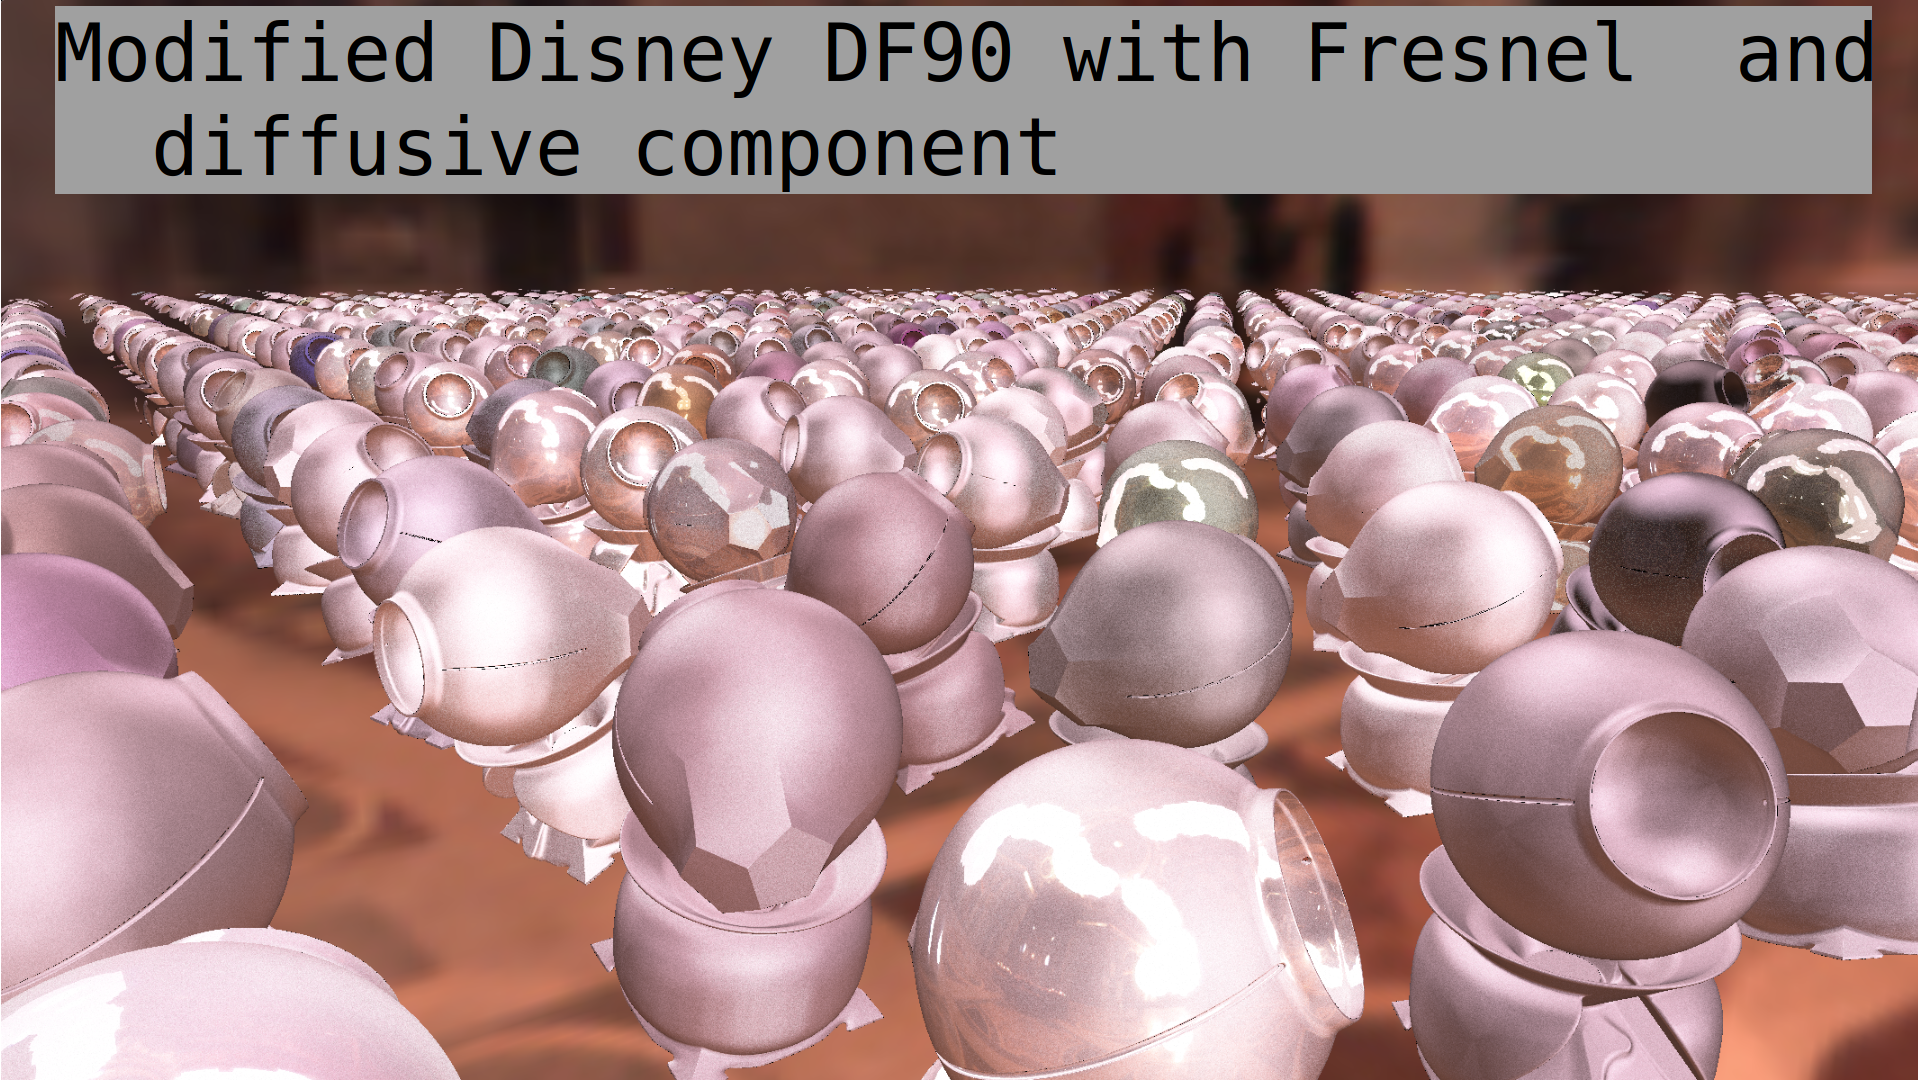
\includegraphics[scale=0.20]{fresnel}
  
  The Geometric term is used to control how microfacets 'shadow' each other. The DTQ BRDF uses Heits' [2014] SmithGGXCorrelated modified to use a half vector, combined with an anisotropic term based off the GGX Anisotropic model:
  \begin{lstlisting}
  const float Param  = sqr(0.5f + sqr(m->roughness)),
  Aspect = sqrt(1.0f - m->anisotropic*0.9f),
  Ax     = Param/Aspect, Ay = Param*Aspect,
  GGX_NV = Smith_G_GGX_Correlated(cos_HL, cos_NV, Ax),
  GGX_HL = Smith_G_GGX_Correlated(cos_NV, cos_HL, Ay);
  microfacet *= 0.5f / (GGX_NV*Ax + GGX_HL*Ay);
  \end{lstlisting}
  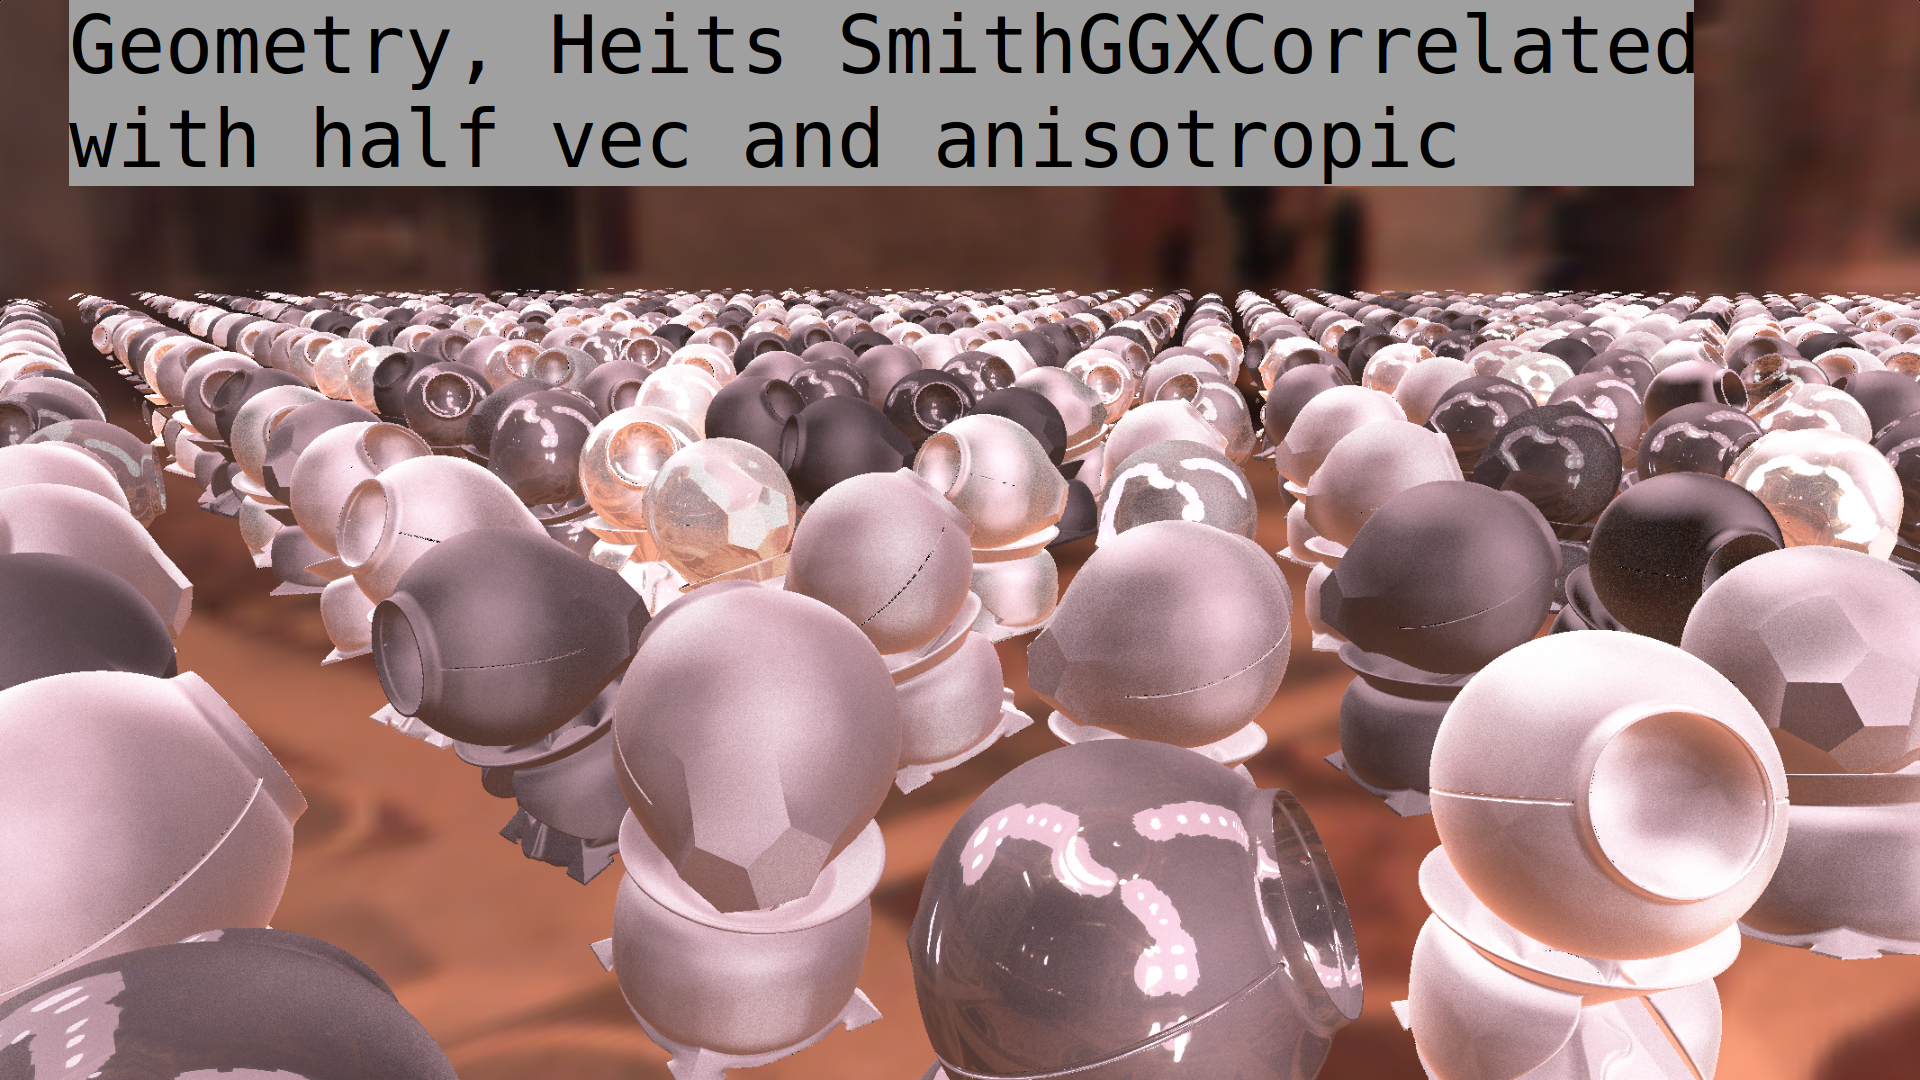
\includegraphics[scale=0.20]{geometric}
  
  And finally, the Distribution term controls how microfacets are spread around the normal. It's based off the Hyper Cauchy with a roughness and metallic (shape) parameters [9]. The latter of which should most likely be its own parameter in the future. The more readable mathematical model is shown:
  
  \begin{align}
  \frac{(M - 1)\:(\sqrt{2})^{2\:S\:-\:2}}
  	    {\pi\:R^{2}\:cos^{4}\theta\:(2 +
  	      \frac{tan^{2}\theta}{M^2})^M}
  \end{align}
  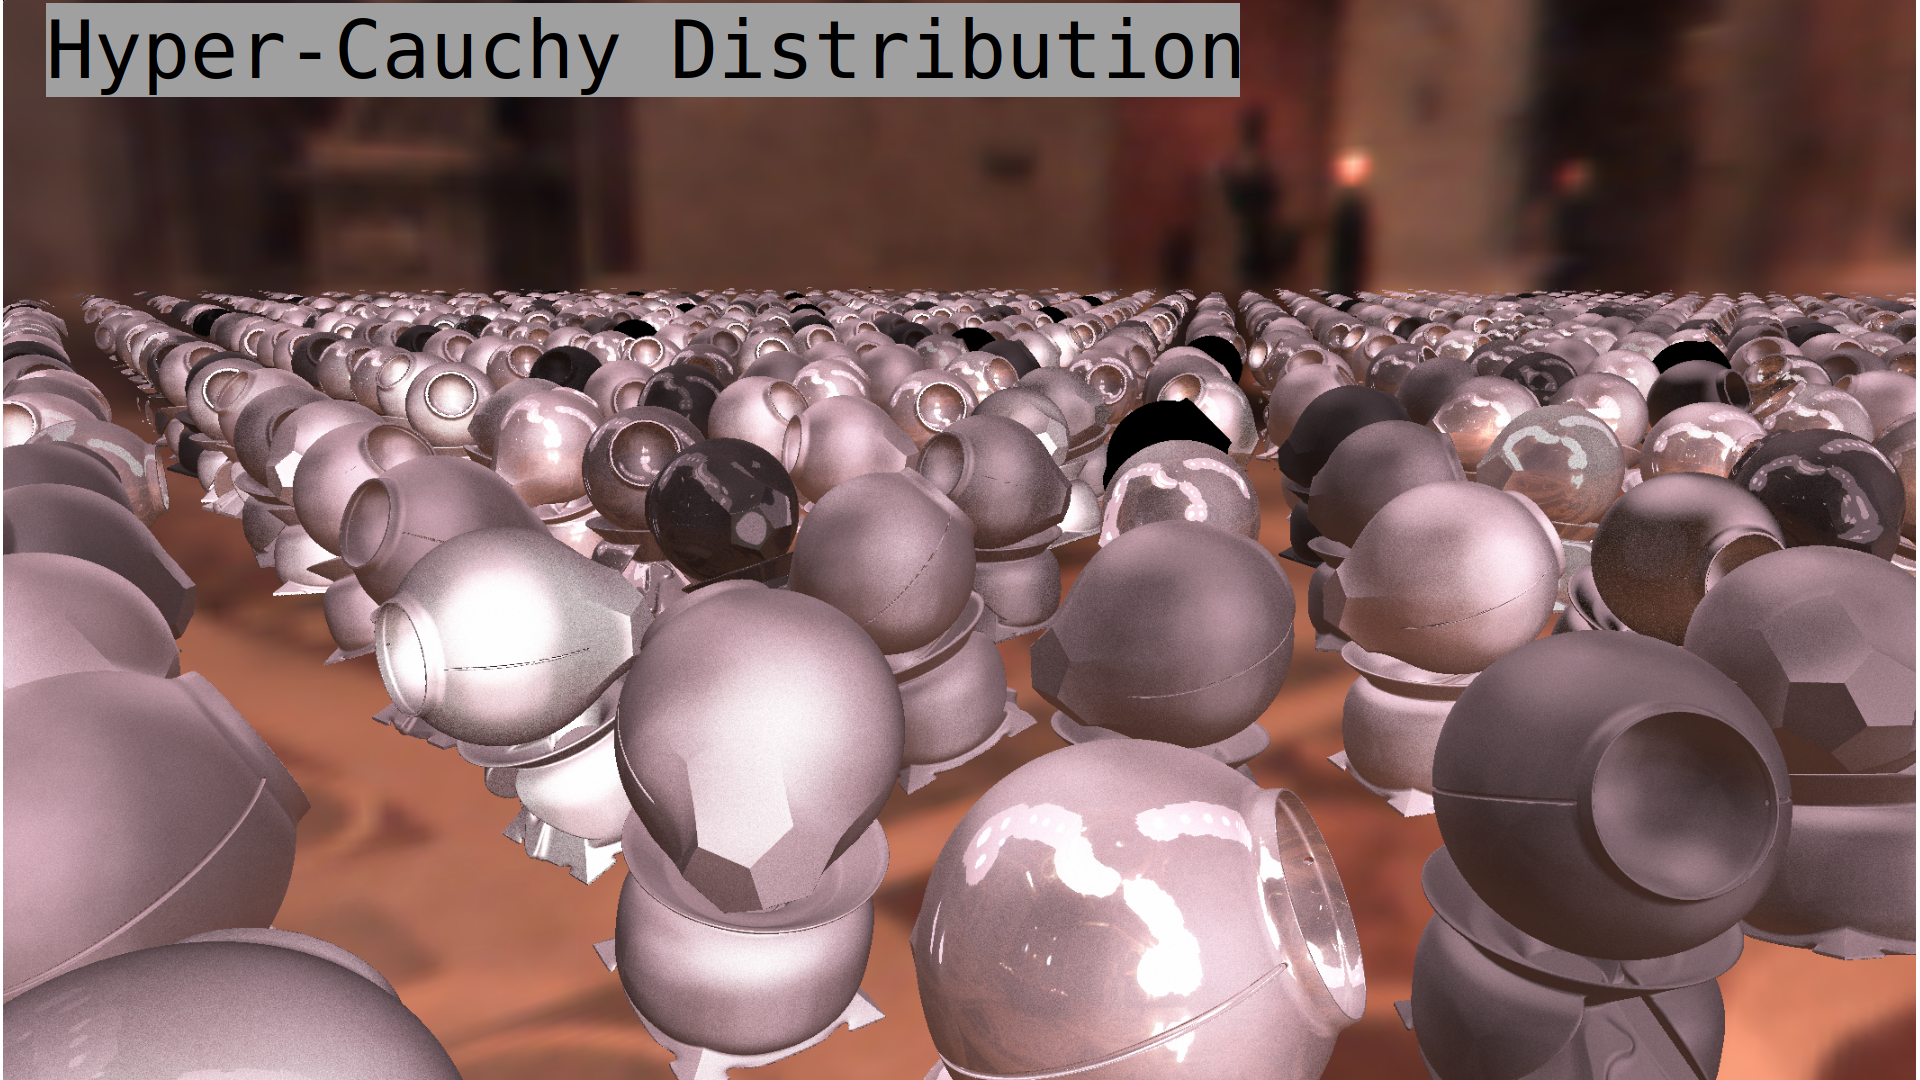
\includegraphics[scale=0.20]{distribution}
  
  These combine to form the microfacet under the half vector microfacet energy conservation model [Edwards et al. 2006].
  \[
  	\frac{F*G*D}{4 \: (H \cdot V) \: ( (N \cdot L) \vee (N \cdot V) )}
  \]
  
  The diffusive component is a combination of both the subsurface and lambertian component. The lambertian is simply $\alpha^{0.5} * \frac{1}{\pi}$, and the subsurface component is based off the Henyey-Greenstein formula [Henyey], modified for half-vec:
  \begin{align}
  	\frac{m(1 - r^2)}{4\pi}\:\frac{1}{(1 + r^2 - 2\:r\:
  		(H \cdot V))^{3/2}}
  \end{align}
  where m is metallic and r is roughness. This is then combined to the diffusive component of the BRDF using Fresnel factor like so:
  \begin{lstlisting}
const float R = (-0.3f + 1.3f*m->roughness)*cos_HV,
            M = (1.0f - m->metallic)*5.0f;
const float Rr_term = M * (1.0f - sqr(R))*IPI *
                      (1.0f/(pow(1.0f + sqr(R) - 2.0*R*cos_HL, 3.0f/2.0f)));
const float3 Retro_reflection = diffusive_albedo * Rr_term *
                  (Fresnel_L + Fresnel_V + (Fresnel_L*Fresnel_V*(Rr_term)));
diffusive_albedo = mix(diffusive_albedo, Retro_reflection, m->subsurface);

  \end{lstlisting}
  TODO: With 0.95 to exaggerate
  
  The microfacet and diffusive components are then added together.

  \section{Video/Image Emitter}

  \section{Future Improvements}

  Every emitter is chosen uniformly, however a better system would weight the
  probability of each emitter by
  \[
    p_l = \frac{\phi_lr_l}{\Sigma_i\phi_ir_l}
  \]
  Thus emitters that have a higher contribution to the scene, that is, a larger
  emittance and radius, will have a higher probability to be selected.

 
        // What's defined: V1 -> V2 [we're evaluating V1] This is for a lens.
        // So, it's ultimately completely useless until an
        // actual lens exists in the SDF scene. Note that this isn't an actual
        // point on a surface of the scene (that's V2, next up for eval), this
        // is just an infinitesimal point based off where the camera currently
        // is, just like a delta light. So while the point actually exists on a
        // scene, the evaluation is on a "delta camera"
  
  \section{Bibliography}
  [1]
  \begin{align*}
    \Sigma_{k=1}^{\infty} \int_{M^{k+1}} L_e(v_0 \rightarrow v_1) G(v_0
    \leftrightarrow v_1)
    \Pi_{i=1}^{k-1} F_s(v_{i-1} \rightarrow v_i \rightarrow v_{i+1}) G(v_i
    \leftrightarrow v_{i+1})\\
    W_e^j(v_{k-1} \rightarrow v_k) dA(v_0) \ldots dA(v_k)
  \end{align*}
  [9]
  Samuel D. Butler, Experimental and Theoretical Basis for a closed-Form Spectral BRDF model
  
  [Henyey]
   Diffuse Radation in the Galaxy, 1942. L, G. Henyey and J. L. Greenstein. 
\end{document}